% ==================================================
% CHAPTER 4: The x-ray method
% ==================================================

% Edit count: Lia - 0, Brigitte - 0
\chapter{The x-ray method}
\label{chap:x_ray}

After quadruplets arrived at CERN and were assembled into wedges, a sample of absolute local offsets on each layer were measured using the x-ray method\cite{lefebvre_precision_2020}. An x-ray gun is attached to the source plate glued to the surface of the wedge, as shown in figure~\ref{fig:xray_setup}.

\begin{figure}
    \centering
    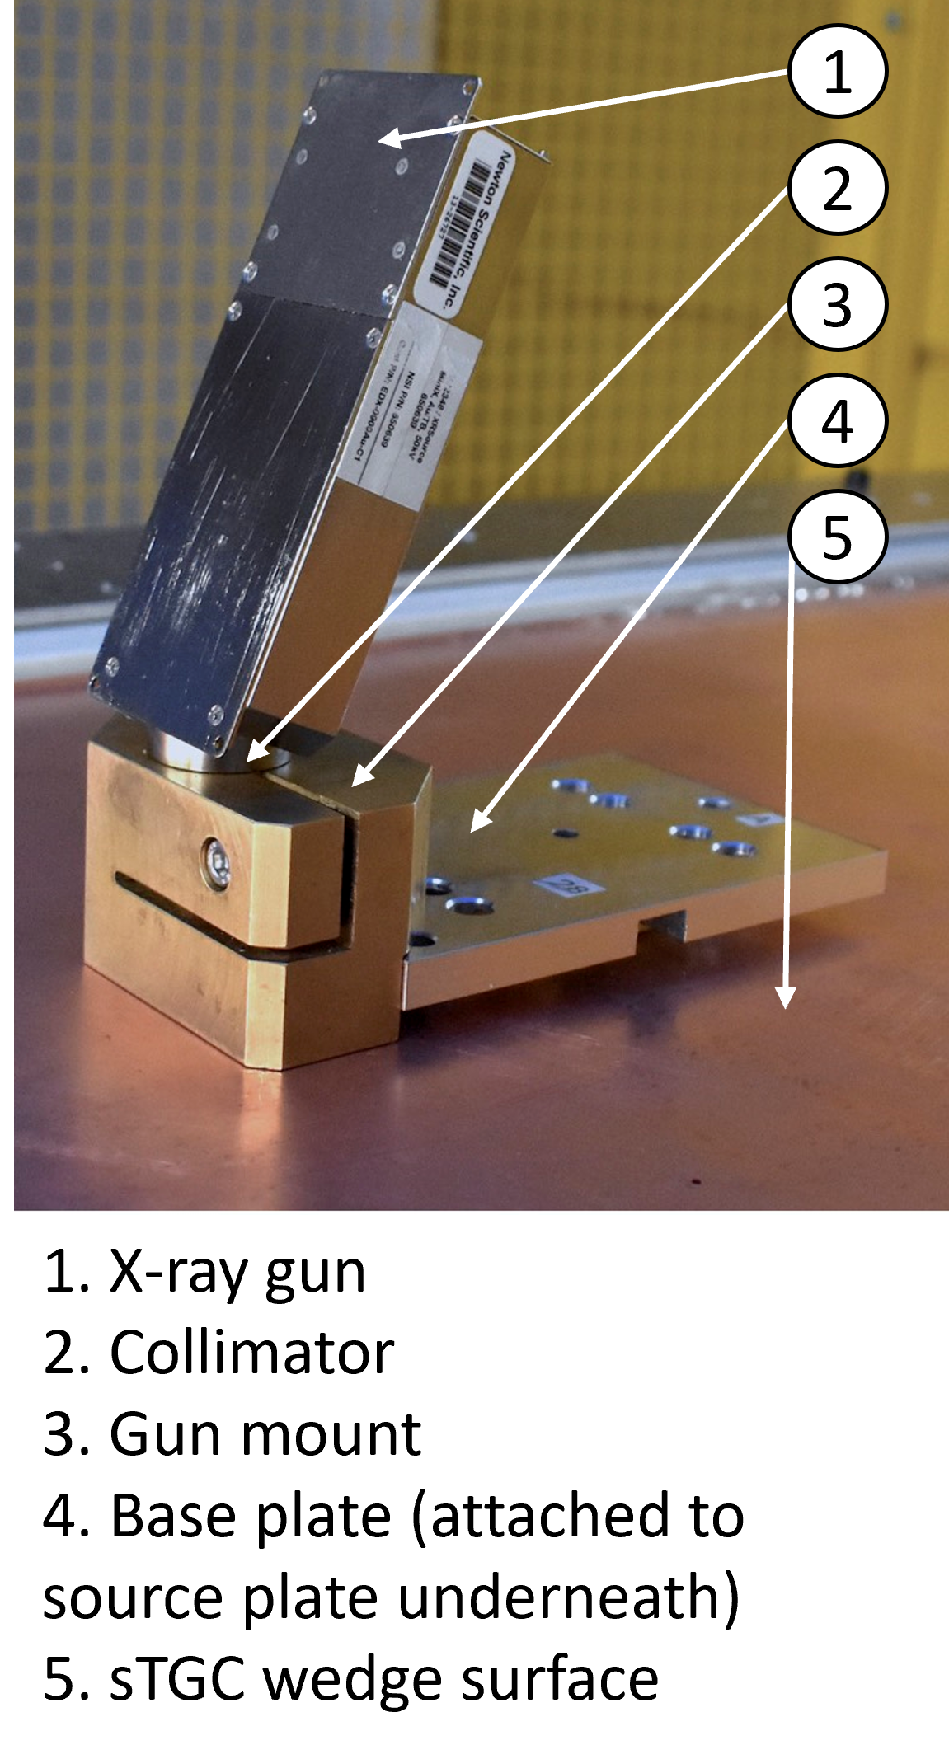
\includegraphics[width = 0.5\textwidth]{figures/figure_xray_setup.pdf}
    \caption{The x-ray gun mounted to the alignment platform on the surface of the wedge. Figure adapted from Lefebvre, 2020~\cite{lefebvre_precision_2020}.}
    \label{fig:xray_setup}
\end{figure}

During operation, the postion of the source plates is monitored via light fibres glued to the wedge surface being monitors by BCAMs on the alignment bars of the new small wheel. Therefore, their position is known in the absolute ATLAS coordinate system. 

When the gun is turned on, electrons strike a gold target in the gun to produce x-rays with energies between 7 and 15 keV, which are passed through the collimator and interact with the materials in the sTGC wedge. The x-rays mostly interact via the photo effect with the copper electrodes and gold-plated tungsten wires. The resulting photoelectrons then ionize the CO$_2$ in the gap, which results in detectable townsend avalanches. 

% To talk about: 
% How the x-rays interact with the chamber
% How we get absolute local offsets.